\section{The QuickDough Overlay} \label{sec:scgraimplement}
One key factor that determines the accelerator's performance rests on the design of the overlay.
While the use of an overlay improves compilation speed and designers' productivity, the QuickDough
framework will not be as useful without significant performance speedup. For that, QuickDough chose
to utilize an overlay that is \emph{simple}, \emph{scalable} and \emph{deterministic}.

The QuickDough overlay consists of an array of simple processing elements (PEs) connected by a
direct network executing synchronously (\figref{fig:scgra-accelerator}).
Each PE computes and forwards data in lock steps, allowing deterministic multi-hop data
communication that overlaps with computations.
The action of each PE in each cycle is controlled by an instruction ROM that is populated with
instructions generated by the compiler.
Finally, a data memory is featured on each PE to serve as a temporary storage for run-time data that
may be reused in the same PE or be forwarded in subsequent steps.


%One key idea of QuickDough is to rely on an intermediate SCGRA overlay to improve compilation time of the high-level user application. While the exact design of this SCGRA does not affect the compilation flow, its implementation does have a significant impact on the performance of the generated gateware.


%% I/O
Communication between the accelerator and the host processor is carried through a group of input/output buffers.
Accesses to these I/O buffers from the SCGRA array take place in lock step with the rest of the system.
The exact buffer location to be accessed is control by the AddrIBuf and AddrOBuf blocks.  Both of them are ROM populated with address information generated from the QuickDough compiler.


%% Reconfiguration
\subsection{Reconfiguration}
There are two levels of reconfiguration that may be applied to the overlay to address different application needs.  The first and the quickest form of reconfiguration keeps the physical implementation of the overlay intact.
To modify the function of the implemented hardware, the QuickDough overlay can be configured by changing (i) the content of the instruction ROM of each PE, (ii) the content of the input/output buffer,  (iii) the content of the I/O buffer address ROM AddrIBuf and AddrOBuf, and (iv) the accelerator control AccCtrl.  Among these 4 aspects, (i) and (iii) are modified by replacing the ROM content of the bitstream in-place using tools such as \texttt{data2mem}.  On the other hand (ii) and (iv) are controlled by software during run-time.  As a result, all 4 types of customization can be performed rapidly within seconds.  They allow the same overlay implementation to be targeted to different applications as well as to different loop iterations of the compute kernel easily.

A second level of customization can be applied to the overlay implementation itself.
As a \emph{soft} overlay, many aspects of the array can be customized according to the input application to achieve different tradeoffs in area, power and performance.  Customizations may involve, the size of the array, the type of supported operation in each PE, the size of data and instruction memory, and even the pipeline depth of the network and the PEs.  
When compared to the first level of customization, this level of customization involves reimplementation of the overlay and requires considerably longer run time.
User may therefore opt for this level of customization only as needed.
Note that in all cases, the overlay remains synchronous and deterministic to keep the overall flow of QuickDough intact.


%\subsection{SCGRA Based FPGA Accelerator}
%\figref{fig:FPGA-accelerator} presents the proposed FPGA accelerator built on top of an SCGRA overlay. The input/output data buffers and Acc-Ctrl block are the same with those in the typical acceleration architecture in \figref{fig:typical-FPGA-accelerator}, while the computation core is unique. It consists of an array of synchronous PEs which can be easily pipelined and run at higher frequency. Moreover, the regular array is able to maintain the high implementation frequency even when it scales up.

%On top of the computation core, the accelerator has two address buffers (Addr IBuf/OBuf) instead of customized logic to control the on-chip data buffer accessing. When target application changes, the user can simply update the content of the address buffers to adapt to the change and thus can reuse the same hardware structure, which is beneficial to design reuse and improving design productivity. 

%Another important block of the accelerator is SCGRA-Ctrl. It can be used to iterate the SCGRA execution until the executions consume all the data in input data buffer or fill the output data buffer. As the executions can share the same input/output data buffer, it helps to increase the data reuse and reduce the communication cost. 

%\begin{figure}[htb]
%    \center{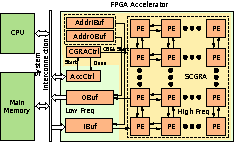
\includegraphics[width=0.6\linewidth]{scgra-accelerator}}
%    \caption{SCGRA Overlay Based FPGA Accelerator}
%    \label{fig:scgra-accelerator}
%\end{figure}
% \begin{figure}[htpb]
% \centering
% \subfloat[]{
% \label{fig:scgra-accelerator}
% 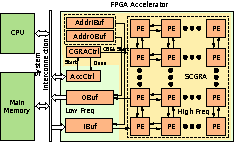
\includegraphics[width=0.6\linewidth]{scgra-accelerator}}
% \qquad
% \subfloat[]{
% \label{fig:hls-accelerator}
% \includegraphics[width=0.6\linewidth]{hls-accelerator}}
% \caption{SCGRA Based FPGA Accelerator and HLS Based FPGA Accelerator}
% \label{fig:FPGA-accelerator}
% \end{figure}

\subsection{Processing Element (PE)}
The key design element of the QuickDough overlay is its processing element (PE).
On one hand, the design of the PE must be simple with low overhead to reduce area and power consumption, and to improve performance.
On the other hand, the design of PE must also be flexible enough that it can support all required operations in the target application.

\begin{figure}
\center{\includegraphics[width=0.6\linewidth]{pe}}
\caption{Fully pipelined PE structure. Each PE can be connected to at most 4 neighbours.}
\label{fig:pe}
\end{figure}

\figref{fig:pe} shows the current implementation of a QuickDough PE that features an optional load/store path. 
At the heart of the PE is an ALU, which is supported by a multi-port data memory and an instruction memory.
Three of the data memory's read ports are connected to the ALU as inputs, while the remaining ports are sent to the output multiplexors for connection to neighboring PEs and the optional store path to OBuf external to the PE.
At the same time, this data memory takes input from the ALU output, data arriving from neighboring PEs, as well as from the optional IBuf loading path.
The action of the PE is controlled by the AddrCtrl unit that reads from the instruction memory.
Finally, a global signal from the AccCtrl block controls the start/stop of all PEs in the array.


\subsubsection{Instruction Memory and Data Memory}
The instruction memory stores all the control words of the PE.  As its content does not change at runtime, a ROM is used to implement this instruction memory. The address of the instruction ROM is determined by the AddrCtrl. Once the global
%\signal{start}
\texttt{start}
signal is valid, the ROM address will increase by one every cycle and the SCGRA execution will proceed accordingly. When the start signal is invalid, the ROM address will be reset to be 0 and the SCGRA execution will stop.

Data memory stores intermediate data that can either be forwarded to the neighboring PEs or be sent to the ALU for calculation.
To support non-blocking operations in the PE, at least 4 read and 2 write ports are needed.  In each cycle, 3 reads are needed for the ALU and 1 read is needed for data forwarding.  At the same time, one write port is needed to store input data from neighboring PEs and another one is needed to store the computing result of the ALU within the same cycle.
%Although a pair of true dual port memories seem to meet this port requirement, conflicts may arise if the ALU needs to read the data while the data path needs to be written. As a result, a third dual port memory is added to the data memory.
%
Currently, 3 true dual port memory blocks that contain replicated data are employed to implement this data memory.

\subsubsection{ALU}
At the heart of the proposed PE is the ALU that carries out the computations of the given application.  As an overlay, the QuickDough ALU must be simple, regular, and flexible such that it may easily be customized with different operations specifically for any given user application.  In addition, it must also be fully pipelined in order to achieve high clock frequency and thus higher overall performance.  \figref{fig:ALU} shows the current design of the ALU used in the QuickDough overlay.

\begin{figure}
\center{\includegraphics[width=0.49\linewidth]{alu-v2}}
\caption{The QuickDough ALU. It supports up to 16 fully pipelined 3-input operations.}
\label{fig:ALU}
\end{figure} 

The QuickDough ALU supports up to 16 fully pipelined 3-input operations.  Depending on the area-performance requirements, the ALU may be customized with operations specifically designed for the application.  It may also be customized to support the common set of operations for multiple compute kernels. For example, \tabref{tab:operations} shows the set of operations we have developed for all the benchmarks in \secref{sec:experiments}.  \figref{fig:ALU} shows the current set of operation.

These operators in the ALU may execute concurrently in a pipelined fashion and must complete in a deterministic number of cycle.  Given the deterministic nature of the operators, the QuickDough scheduler will ensure that there is never conflict at the output multiplexor.

%To customize the ALU, one may replace any of the available slot with a new customized operation.  The QuickDough compiler should also be notified of this new operation so it would extract the corresponding operation in the DFG, and generate the correct instruction. 

%It involves a number of fully pipelined data paths with variable pipeline stages and applies Sel signal from instruction ROM directly for output selection. As the scheduler will make sure that there is no output conflict, opcode decoding logic used in conventional ALU is removed. 

% mine
%\figref{fig:ALU} shows the ALU design that was used in the experiments for this work.
%It supports a set of operations shown in \tabref{tab:operations} that is sufficient to implement all benchmark applications in this work without reimplementing the physical hardware.
%It is important to note that this list of supported operations in the ALU is part of the customizable feature of the overlay.
%[HHH do we have work to show how customized instruction work?]
%Regardless of the operation set, a common design choice for the QuickDough overlay ALU is that it supports 3 input operands.
%It was designed like this such that it can easily support the multiply-add operation commonly found in many data intensive operations.
%The rest of the operation set as shown in \tabref{tab:operations} is therefore created such that they all take advantage of the 3 inputs.
%Finally, the DFG generation step ensures it will take advantage of these 3-input operations.


% shows an example design that can support all the operations of our benchmark as listed in \tabref{tab:operations}. In order to make full use of the Multiplication-Addition IP core on FPGA, MULADD/SUB is involved in ALU and there are three read ports connected to ALU. In this case, we will not waste the bandwidth of data memroy, and we tend to use three source opernds while generating the DFGs. 

%As the operations are usually different, each operation is provided with an independent data path. At the end of the data paths, a set of multiplexers are added to select the expected output. Currently, the maximum number of operations allowed in this template is 16 and an additional pipeline stage is added for the output selection. As the scheduler will make sure that the output port of the ALU is contention-free, the opcode in this ALU doesn't have to align with the input operations. Instead, it is merely used for output selection. Therefore, the proposed ALU can be easily customized and scaled.


\begin{table}
\tbl{Operation Set Implemented in ALU. It covers all the four applications used in the experiments.\label{tab:operations}}{
\footnotesize 
\centering
\resizebox{0.5\columnwidth}{!}{
\begin{tabular}{l|c|l}
\hline
Type & Opcode & Expression \\

\hline
MULADD & 0001 & {Dst = (Src0 $\times$ Src1) + Src2} \\

\hline
MULSUB & 0010 & {Dst = (Src0 $\times$ Src1) - Src2} \\

\hline
ADDADD & 0011 & {Dst = (Src0 + Src1) + Src2} \\

\hline
ADDSUB & 0100 & {Dst = (Src0 + Src1) - Src2} \\

\hline
SUBSUB & 0101 & {Dst = (Src0 - Src1) - Src2} \\

\hline 
PHI & 0110 & {Dst = Src0 ? Src1 : Src2} \\

\hline
RSFAND & 0111 & {Dst = (Src0 $\gg$ Src1) \& Src2} \\

\hline
LSFADD & 1000 & {Dst = (Src0 $\ll$ Src1) + Src2} \\

\hline
ABS & 1001 & {Dst = abs(Src0)} \\

\hline
GT & 1010 & {Dst = (Src0 $>$ Src1) ? 1 : 0} \\

\hline
LET & 1011 & {Dst = (Src0 $\leq$ Src1) ? 1 : 0} \\

\hline
ANDAND & 1100 & {Dst = (Src0 \& Src1) \& Src2} \\

\hline
\end{tabular}
}
}
\end{table}

\subsubsection{Load/Store Interface}
For the PEs that also serve as IO interface to the SCGRA, they have an additional load path and a store path as shown in \ref{fig:pe}. The data loading path and the SCGRA neighboring input share a single data memory write port, and an additional pipeline stage is added to keep the balance of the pipeline.
Similarly, the data storing path has an additional data multiplier as well, but it doesn't influence the pipeline of the design. 

\subsection{Input/Output Buffer}
Input/output buffer is used to store data transmitted between the FPGA 
accelerator and main memory. (The input and output buffers are quite similar, so 
we just present the input buffer structure here.) 
It is usually implemented with block RAM and 
a naive implementation as shown in \figref{fig:naive-implementation} 
provides limited bandwidth to the computing logic and may dramatically 
restrict the performance of the accelerator. A straightforward solution is to 
expose the primitive block RAM ports to the accelerator 
directly as shown in \figref{fig:quick-partition}. However, the bandwidth is 
limited by the number of the primitive block RAM and it works only when 
the data is perfectly placed into different block RAM banks and each port of 
the accelerator accesses exactly the corresponding sub set of the data. However, 
we may have the input/output data of iterated DFGs extracted from the same loop stored in the
input/output buffers when transmitted from/to main memory to amortize the initial communication
cost, while different input/output of the DFGs may have diverse layout pattern. For instance, one DFG 
may load its first input data from partitioned bank 0 while the 
following DFG may have to load its first input data from bank 1. As a result, 
the two DFGs will not be able to reuse the same lock-step computing on the SCGRA overlay and
providing each DFG with different scheduling will be extremely expensive.

To solve this problem, we have introduced an additional buffering stage and developed 
a scalable on-chip buffer structure as shown in \figref{fig:scalable-partition1} 
and \figref{fig:scalable-partition2}. The first stage is the basic on-chip buffer as 
mentioned in \figref{fig:naive-implementation} and \figref{fig:quick-partition}. It stores 
data transmitted between the accelerator and main memory. The additional 
buffer stage stores the input/output of the DFG computation on the SCGRA overlay. It ensures the 
input/output data has exactly the same layout for all the iterated DFG computation and can be 
implemented with arbitrary number of partitions providing sufficient bandwidth to the computing
logic. 

\begin{figure}[tb]
    \centering
	\subfloat[Naive buffer structure]{%
		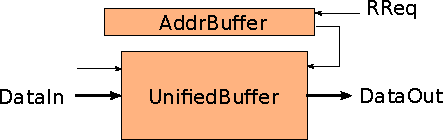
\includegraphics[width=0.3\textwidth]{buffer-type0}
        \label{fig:naive-implementation}
	}\qquad
	\subfloat[Partitioned buffer structure]{%
		\includegraphics[width=0.35\textwidth]{buffer-type1}
        \label{fig:quick-partition}
	}
    \hfill
	\subfloat[Naive partitioned two-stage buffer structure]{%
		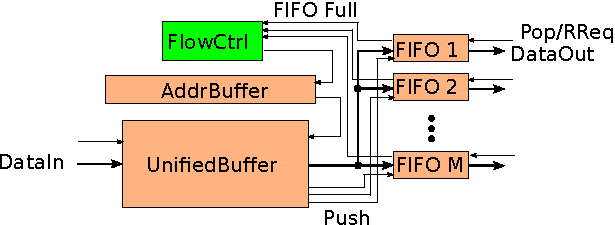
\includegraphics[width=0.45\textwidth]{buffer-type2}
        \label{fig:scalable-partition1}
	}
	\subfloat[Generic partitioned two-stage buffer structure]{%
		\includegraphics[width=0.55\textwidth]{buffer-type3}
        \label{fig:scalable-partition2}
	}
    \caption{Input/output buffer structure}
	\label{fig:on-chip-buffer}
\end{figure}

Although the additional buffer stage makes the computation data path even 
longer, data movement between the first buffer stage and the second buffer 
stage and the iterated DFG computing can be pipelined as illustrated in \figref{fig:buffer-pipelining}. 
As long as the second stage buffers are not full, FlowCtrl will keep the 
first stage buffer sending data to the second buffer stage with the 
pre-scheduled order which can be obtained from the SCGRA overlay scheduling 
and stored in the AddrBuffer. When the second buffer stage has all the input for a 
single DFG execution, FlowCtrl will start the accelerator. When the 
accelerator completes a DFG computing, it will stop until it is activated 
next time. On the output side, the buffer and the accelerator work similarly.
When the number of the iterated DFGs is large enough and DFG computing 
time is larger than the data movement cost, the cost of the 
additional buffer stages can be ignored. In addition,  
to ensure the pipelining in \figref{fig:buffer-pipelining}, 
the second buffer stage capacity is set to be twice the input/output 
of a single DFG. 

\begin{figure}[tb]
\center{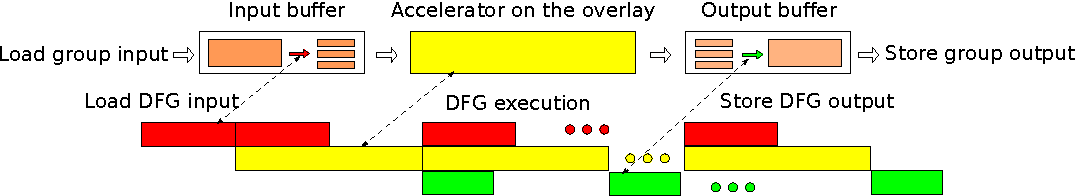
\includegraphics[width=0.9\linewidth]{buffer-pipelining}}
\caption{Pipelined execution on the SCGRA overlay}
\label{fig:buffer-pipelining}
\end{figure}


